% Options for packages loaded elsewhere
\PassOptionsToPackage{unicode}{hyperref}
\PassOptionsToPackage{hyphens}{url}
\PassOptionsToPackage{dvipsnames,svgnames,x11names}{xcolor}
%
\documentclass[
  a4paper,
]{scrreport}

\usepackage{amsmath,amssymb}
\usepackage{iftex}
\ifPDFTeX
  \usepackage[T1]{fontenc}
  \usepackage[utf8]{inputenc}
  \usepackage{textcomp} % provide euro and other symbols
\else % if luatex or xetex
  \usepackage{unicode-math}
  \defaultfontfeatures{Scale=MatchLowercase}
  \defaultfontfeatures[\rmfamily]{Ligatures=TeX,Scale=1}
\fi
\usepackage{lmodern}
\ifPDFTeX\else  
    % xetex/luatex font selection
\fi
% Use upquote if available, for straight quotes in verbatim environments
\IfFileExists{upquote.sty}{\usepackage{upquote}}{}
\IfFileExists{microtype.sty}{% use microtype if available
  \usepackage[]{microtype}
  \UseMicrotypeSet[protrusion]{basicmath} % disable protrusion for tt fonts
}{}
\makeatletter
\@ifundefined{KOMAClassName}{% if non-KOMA class
  \IfFileExists{parskip.sty}{%
    \usepackage{parskip}
  }{% else
    \setlength{\parindent}{0pt}
    \setlength{\parskip}{6pt plus 2pt minus 1pt}}
}{% if KOMA class
  \KOMAoptions{parskip=half}}
\makeatother
\usepackage{xcolor}
\setlength{\emergencystretch}{3em} % prevent overfull lines
\setcounter{secnumdepth}{5}
% Make \paragraph and \subparagraph free-standing
\ifx\paragraph\undefined\else
  \let\oldparagraph\paragraph
  \renewcommand{\paragraph}[1]{\oldparagraph{#1}\mbox{}}
\fi
\ifx\subparagraph\undefined\else
  \let\oldsubparagraph\subparagraph
  \renewcommand{\subparagraph}[1]{\oldsubparagraph{#1}\mbox{}}
\fi


\providecommand{\tightlist}{%
  \setlength{\itemsep}{0pt}\setlength{\parskip}{0pt}}\usepackage{longtable,booktabs,array}
\usepackage{calc} % for calculating minipage widths
% Correct order of tables after \paragraph or \subparagraph
\usepackage{etoolbox}
\makeatletter
\patchcmd\longtable{\par}{\if@noskipsec\mbox{}\fi\par}{}{}
\makeatother
% Allow footnotes in longtable head/foot
\IfFileExists{footnotehyper.sty}{\usepackage{footnotehyper}}{\usepackage{footnote}}
\makesavenoteenv{longtable}
\usepackage{graphicx}
\makeatletter
\def\maxwidth{\ifdim\Gin@nat@width>\linewidth\linewidth\else\Gin@nat@width\fi}
\def\maxheight{\ifdim\Gin@nat@height>\textheight\textheight\else\Gin@nat@height\fi}
\makeatother
% Scale images if necessary, so that they will not overflow the page
% margins by default, and it is still possible to overwrite the defaults
% using explicit options in \includegraphics[width, height, ...]{}
\setkeys{Gin}{width=\maxwidth,height=\maxheight,keepaspectratio}
% Set default figure placement to htbp
\makeatletter
\def\fps@figure{htbp}
\makeatother

%\newfontfamily\Ubuntu[Mapping=tex-text]{Ubuntu}
\usepackage{pgfplots}
\usetikzlibrary{arrows.meta,arrows}
\usetikzlibrary{angles,quotes}
\pgfplotsset{grid style={dashed,mygray}}
% Colors
\definecolor{myblue}{rgb}{0.067,0.529,0.871}
\definecolor{mypurple}{rgb}{0.859,0.071,0.525}
\definecolor{myred}{rgb}{1.0, 0.13, 0.32}
\definecolor{mygreen}{rgb}{0.01, 0.75, 0.24}
\definecolor{myblack}{gray}{0.1}
\definecolor{mygray}{gray}{0.8}
\newcommand{\NN}{\mathbb{N}}
\newcommand{\ZZ}{\mathbb{Z}}
\newcommand{\QQ}{\mathbb{Q}}
\newcommand{\RR}{\mathbb{R}}
\newcommand{\CC}{\mathbb{C}}
\DeclareMathOperator{\operatorname{Int}}{Int}
\DeclareMathOperator{\operatorname{Ext}}{Ext}
\DeclareMathOperator{\operatorname{Fr}}{Fr}
\DeclareMathOperator{\Adh}{Adh}
\DeclareMathOperator{\Ac}{Ac}
\DeclareMathOperator{\sen}{sen}
\makeatletter
\makeatother
\makeatletter
\@ifpackageloaded{bookmark}{}{\usepackage{bookmark}}
\makeatother
\makeatletter
\@ifpackageloaded{caption}{}{\usepackage{caption}}
\AtBeginDocument{%
\ifdefined\contentsname
  \renewcommand*\contentsname{Tabla de contenidos}
\else
  \newcommand\contentsname{Tabla de contenidos}
\fi
\ifdefined\listfigurename
  \renewcommand*\listfigurename{Listado de Figuras}
\else
  \newcommand\listfigurename{Listado de Figuras}
\fi
\ifdefined\listtablename
  \renewcommand*\listtablename{Listado de Tablas}
\else
  \newcommand\listtablename{Listado de Tablas}
\fi
\ifdefined\figurename
  \renewcommand*\figurename{Figura}
\else
  \newcommand\figurename{Figura}
\fi
\ifdefined\tablename
  \renewcommand*\tablename{Tabla}
\else
  \newcommand\tablename{Tabla}
\fi
}
\@ifpackageloaded{float}{}{\usepackage{float}}
\floatstyle{ruled}
\@ifundefined{c@chapter}{\newfloat{codelisting}{h}{lop}}{\newfloat{codelisting}{h}{lop}[chapter]}
\floatname{codelisting}{Listado}
\newcommand*\listoflistings{\listof{codelisting}{Listado de Listados}}
\usepackage{amsthm}
\theoremstyle{definition}
\newtheorem{exercise}{Ejercicio}[chapter]
\theoremstyle{remark}
\AtBeginDocument{\renewcommand*{\proofname}{Prueba}}
\newtheorem*{remark}{Observación}
\newtheorem*{solution}{Solución}
\makeatother
\makeatletter
\@ifpackageloaded{caption}{}{\usepackage{caption}}
\@ifpackageloaded{subcaption}{}{\usepackage{subcaption}}
\makeatother
\makeatletter
\@ifpackageloaded{tcolorbox}{}{\usepackage[skins,breakable]{tcolorbox}}
\makeatother
\makeatletter
\@ifundefined{shadecolor}{\definecolor{shadecolor}{rgb}{.97, .97, .97}}
\makeatother
\makeatletter
\makeatother
\makeatletter
\makeatother
\ifLuaTeX
\usepackage[bidi=basic]{babel}
\else
\usepackage[bidi=default]{babel}
\fi
\babelprovide[main,import]{spanish}
% get rid of language-specific shorthands (see #6817):
\let\LanguageShortHands\languageshorthands
\def\languageshorthands#1{}
\ifLuaTeX
  \usepackage{selnolig}  % disable illegal ligatures
\fi
\IfFileExists{bookmark.sty}{\usepackage{bookmark}}{\usepackage{hyperref}}
\IfFileExists{xurl.sty}{\usepackage{xurl}}{} % add URL line breaks if available
\urlstyle{same} % disable monospaced font for URLs
\hypersetup{
  pdftitle={Problemas de Estadística},
  pdfauthor={Alfredo Sánchez Alberca},
  pdflang={es},
  colorlinks=true,
  linkcolor={blue},
  filecolor={Maroon},
  citecolor={Blue},
  urlcolor={Blue},
  pdfcreator={LaTeX via pandoc}}

\title{Problemas de Estadística}
\author{Alfredo Sánchez Alberca}
\date{2022-01-06}

\begin{document}
\begin{titlepage}

%\AddToShipoutPicture*{\put(0,0){\includegraphics[scale=0.8]{img/background2}}} % Imagen de fondo, requiere el paquete eso-pic.
\begin{center}
\vspace*{5cm}

\Huge
{\textbf{\textsf{Problemas de Estadística}}}

\vspace{0.5cm}
\LARGE
{\textbf{\textsf{}}}

\vspace{1.5cm}

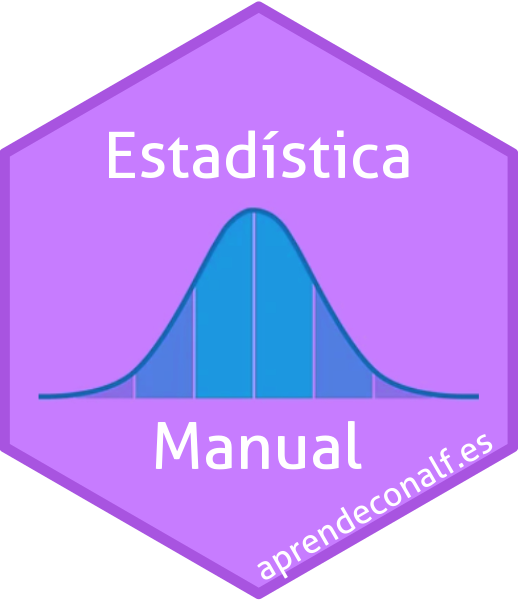
\includegraphics[width=0.4\textwidth]{img/logos/sticker.png}
\end{center}

\vfill

\begin{flushleft}
\begin{tabular}{ll}

\includegraphics[width=0.1\textwidth]{img/logos/aprendeconalf.png} & \parbox[b]{5cm}{\Large\textsf{Alfredo
Sánchez
Alberca}\\ \textsf{asalber@ceu.es} \\ \textsf{https://aprendeconalf.es}}
\end{tabular}
\end{flushleft}
\end{titlepage}\ifdefined\Shaded\renewenvironment{Shaded}{\begin{tcolorbox}[breakable, sharp corners, enhanced, interior hidden, boxrule=0pt, borderline west={3pt}{0pt}{shadecolor}, frame hidden]}{\end{tcolorbox}}\fi

\renewcommand*\contentsname{Tabla de contenidos}
{
\hypersetup{linkcolor=}
\setcounter{tocdepth}{2}
\tableofcontents
}
\bookmarksetup{startatroot}

\hypertarget{prefacio}{%
\chapter*{Prefacio}\label{prefacio}}
\addcontentsline{toc}{chapter}{Prefacio}

\markboth{Prefacio}{Prefacio}

Colección de problemas de Estadística aplicada a la Economía para el
Master en Análisis y Comunicación de Datos.

\bookmarksetup{startatroot}

\hypertarget{estimaciuxf3n-de-paruxe1metros}{%
\chapter{Estimación de
parámetros}\label{estimaciuxf3n-de-paruxe1metros}}

\begin{exercise}[]\protect\hypertarget{exr-distribucion-media-trabajadores-pymes}{}\label{exr-distribucion-media-trabajadores-pymes}

El número medio de trabajadores en las PYMES españolas es 5 y su
varianza 4. Realizado un muestreo aleatorio de 16 PYMES.

Calcular:

\begin{enumerate}
\def\labelenumi{\alph{enumi}.}
\item
  La esperanza y varianza de la media muestral.
\item
  La esperanza de la varianza y de la cuasivarianza muestral.
\item
  Mínimo tamaño que ha de tener la muestra para que exista una
  probabilidad mayor o igual al \(95\)\% de que la media muestral se
  desvíe de la media poblacional a lo sumo \(0.25\) unidades.
\item
  Si realizamos un muestreo aleatorio de tamaño \(320\) obtener
  \(P(4.9\leq \bar x \leq 5.2.\).
\end{enumerate}

\end{exercise}

\begin{exercise}[]\protect\hypertarget{exr-distribucion-cuasivarianza-iberpapel}{}\label{exr-distribucion-cuasivarianza-iberpapel}

El precio de las acciones de Iberpapel se distribuyen según un modelo
normal \(N(\mu, 2.\), analizar \(16\) sesiones de la Bolsa de Madrid
elegidas aleatoriamente, para calcular la probabilidad de que la
cuasivarianza muestral del precio de las acciones sea mayor o igual que
\(2.136\).

\end{exercise}

\begin{exercise}[]\protect\hypertarget{exr-diferencia-proporciones-votos}{}\label{exr-diferencia-proporciones-votos}

El porcentaje de votantes con preferencia de un determinado partido es
del \(5\)\% en una región \(A\), y el \(10\)\% en otra \(B\).
Consultados \(100\) electores de la región \(A\) y \(150\) de la \(B\),
determinar la probabilidad de que el porcentaje de electores consultados
favorables a dicho partido en la segunda región supere en más de
\(0.02\) al porcentaje de electores favorables a dicho partido en la
primera.

\end{exercise}

\begin{exercise}[]\protect\hypertarget{exr-intervalo-confianza-media-demanda}{}\label{exr-intervalo-confianza-media-demanda}

Una empresa desea estudiar la demanda futura de uno de sus productos,
para lo cual selecciona, mediante muestreo aleatorio simple, a diez de
sus clientes, observando el número de unidades demandadas por ellos:

\begin{longtable}[]{@{}rr@{}}
\toprule\noalign{}
Número de unidades demandadas & Número de clientes \\
\midrule\noalign{}
\endhead
\bottomrule\noalign{}
\endlastfoot
100 & 1 \\
102 & 2 \\
104 & 1 \\
106 & 2 \\
108 & 1 \\
110 & 2 \\
112 & 1 \\
\end{longtable}

\end{exercise}

Suponiendo que la demanda sigue una distribución normal.

\begin{enumerate}
\def\labelenumi{\alph{enumi}.}
\tightlist
\item
  Estimar la demanda media mediante un intervalo de confianza con nivel
  de significación \(0.1\).
\item
  ¿Qué tamaño muestral sería necesario para que el intervalo tuviese un
  error máximo de \(\pm 1\) unidad? :::
\end{enumerate}

\begin{exercise}[]\protect\hypertarget{exr-intervalo-confianza-media-bitcoin}{}\label{exr-intervalo-confianza-media-bitcoin}

Al objeto de determinar la proporción de españoles que poseen la
criptomoneda bitcoin se ha realizado un muestreo aleatorio de \(100\)
españoles, resultando que \(15\) tienen bitcoins.

\begin{enumerate}
\def\labelenumi{\alph{enumi}.}
\item
  Obtener un intervalo de confianza del \(95\)\% para la proporción
  poblacional de españoles que poseen bitcoins.
\item
  ¿A cuántos españoles se debería encuestar para lograr una semiamplitud
  del intervalo de \(0.02\), utilizando un nivel de confianza del
  \(80\)\%?
\end{enumerate}

\end{exercise}

\begin{exercise}[]\protect\hypertarget{exr-intervalo-confianza-proporcion-covid}{}\label{exr-intervalo-confianza-proporcion-covid}

Para conocer la prevalencia de la COVID en una población se ha tomado
una muestra aleatoria de \(500\) personas y se ha observado que \(36\)
tenían COVID. ¿Qué precisión tiene el intervalo de confianza del
\(95\)\% para la proporción de personas infectadas en la población? ¿Qué
tamaño muestral habría que tomar para doblar la precisión del intervalo?

\end{exercise}

\begin{exercise}[]\protect\hypertarget{exr-intervalo-confianza-proporcion-demanda}{}\label{exr-intervalo-confianza-proporcion-demanda}

Una empresa quiere conocer la proporción de clientes dispuestos a
demandar un nuevo producto, para averiguarlo efectúa un muestreo
aleatorio de tamaño \(100\) en el que se obtiene que un \(20\)\% de
ellos estarían dispuestos a comprar el nuevo producto. Determinar el
intervalo de confianza para la proporción poblacional con un grado de
confianza del \(90\)\%.

\end{exercise}

\begin{exercise}[]\protect\hypertarget{exr-intervalo-confianza-media-varianza-gasto-alimentacion}{}\label{exr-intervalo-confianza-media-varianza-gasto-alimentacion}

En una comunidad autónoma, los gastos semanales en alimentación por
unidad familiar se distribuyen según un modelo normal \(N(\mu,\sigma.\).
Realizado un muestreo aleatorio en el que se han consultado a \(21\)
unidades familiares hemos obtenido que el gasto medio semanal muestral
es de \(150\) euros y la cuasidesviación típica semanal muestral es de
\(12\) euros.

\begin{enumerate}
\def\labelenumi{\alph{enumi}.}
\item
  Construir un intervalo de confianza del \(95\)\% para el gasto medio
  semanal poblacional.
\item
  Construir un intervalo de confianza del \(95\)\% para la varianza
  poblacional.
\end{enumerate}

\end{exercise}

\begin{exercise}[]\protect\hypertarget{exr-intervalo-confianza-media-varianza-gasto-porcino}{}\label{exr-intervalo-confianza-media-varianza-gasto-porcino}

Los gastos mensuales en carne de porcino en las familias españolas se
distribuyen según un modelo normal \(N(\mu, \sigma.\). Realizando un
muestreo aleatorio en el que se pregunta a \(20\) unidades familiares,
se obtiene que el gasto medio mensual ha sido de \(170.31\) € y la
cuasidesviación típica de \(36\) €.

\begin{enumerate}
\def\labelenumi{\alph{enumi}.}
\item
  Obtener el intervalo de confianza para el gasto medio mensual en carne
  de porcino con un \(95\)\% de confianza.
\item
  Razone cómo podría obtener un intervalo de confianza más preciso para
  el gasto medio, suponiendo que no varían la media muestral, la
  cuasivarianza muestral y el tamaño de la muestra.
\item
  Obtener el intervalo de confianza para la varianza del gasto mensual
  en carne de porcino con un \(95\)\% de confianza.
\end{enumerate}

\end{exercise}

\begin{exercise}[]\protect\hypertarget{exr-intervalo-confianza-media-peso}{}\label{exr-intervalo-confianza-media-peso}

La OMS ha obtenido una muestra de los pesos de \(50\) niños de entre
\(11\) y \(14\) años, que proporciona una media muestral de \(47\) kg y
una desviación típica muestral de \(11\) kg. Suponiendo que la población
sigue una distribución normal.

\begin{enumerate}
\def\labelenumi{\alph{enumi}.}
\item
  Obtener un intervalo de confianza para la media poblacional con un
  \(95\)\% de nivel de confianza.
\item
  El director de la OMS considera que el intervalo es insatisfactorio,
  pero quiere mantener el nivel de confianza. Por ello decide reducir a
  la mitad la precisión de dicho intervalo (reducir un \(50\)\% el radio
  del intervalo.. En estas condiciones, ¿cuál debería ser el tamaño de
  la muestra para cumplir los objetivos del director?
\item
  Los resultados obtenidos en los análisis anteriores siguen sin
  convencer al director de la OMS y le pide a su equipo que establezca
  un intervalo de confianza para la media poblacional con un \(99\)\% de
  nivel de confianza, manteniendo la misma muestra del ejercicio
  anterior.
\item
  El director decide reducir en un tercio la precisión del intervalo
  anterior, pero quiere mantener el nivel de confianza ¿cuál debería ser
  el tamaño de la muestra para cumplir dicho objetivo?
\end{enumerate}

\end{exercise}

\begin{exercise}[]\protect\hypertarget{exr-intervalo-confianza-proporcion-uso-alta-velocidad}{}\label{exr-intervalo-confianza-proporcion-uso-alta-velocidad}

Tras la liberalización del transporte ferroviario de pasajeros en las
líneas de alta velocidad en España, la compañía francesa SNCF estudia la
proporción de clientes que utiliza al menos una vez al mes el servicio
de alta velocidad. A tal efecto la empresa realiza un muestreo aleatorio
en el que se seleccionan \(50\) usuarios y en el que resulta que \(35\)
de ellos afirma utilizar este servicio una vez al mes como mínimo.

Considerando un nivel de confianza del \(98\)\% determine un intervalo
de confianza poblacional para la proporción de usuarios que utilizan la
alta velocidad una vez al mes por lo menos (justifique cómo obtiene el
intervalo de confianza antes de proceder a su cálculo..

\end{exercise}

\bookmarksetup{startatroot}

\hypertarget{contrastes-de-hipuxf3tesis-paramuxe9tricos}{%
\chapter{Contrastes de hipótesis
paramétricos}\label{contrastes-de-hipuxf3tesis-paramuxe9tricos}}

\begin{exercise}[]\protect\hypertarget{exr-contraste-media-consumo-azucar}{}\label{exr-contraste-media-consumo-azucar}

Sabiendo que el año pasado el consumo per cápita de azúcar en España fue
de 4.8 kg y que este consumo sigue una distribución normal, hemos
seleccionado aleatoriamente a 20 españoles obteniendo una media muestral
de 5 kg y una cuasidesviación típica muestral de 0.4 kg. Contrastar la
hipótesis de que el consumo de azúcar per cápita de este año en España
no ha variado utilizando un nivel de significación del 10\% en cada uno
de los casos siguientes.

\begin{enumerate}
\def\labelenumi{\alph{enumi}.}
\item
  Suponiendo que la alternativa es que el consumo de azúcar per cápita
  sea distinto.
\item
  Suponiendo que la alternativa es que el consumo de azúcar per cápita
  sea mayor.
\end{enumerate}

\end{exercise}

\begin{exercise}[]\protect\hypertarget{exr-contraste-proporcion-asistencia-clase}{}\label{exr-contraste-proporcion-asistencia-clase}

En una clase de Estadística se ha comprobado que el 20\% del alumnado
falta a clase. Para disminuir esta preocupante cifra, los profesores han
incorporado un sistema de evaluación continua que tendrá en cuenta las
notas de clase de los alumnos en la nota final. Contraste con un nivel
de significación del 5\% que la incorporación de este método no es
efectiva, es decir, el absentismo antes y después de la evaluación
continua es el mismo, sabiendo que el porcentaje medio de no asistencia
en 50 días tomados al azar ha sido del 17\%.

\end{exercise}

\begin{exercise}[]\protect\hypertarget{exr-contraste-media-detergente}{}\label{exr-contraste-media-detergente}

Una empresa fabricante de detergente afirma que el contenido de cada
paquete de detergente sigue una distribución normal de media 2150 g,
pero una Asociación de Consumidores no está conforme con esta
afirmación, por lo que realiza un estudio consistente en obtener una
muestra aleatoria simple de 121 paquetes de detergente, obteniendo un
contenido medio muestral de 2070 g y una cuasidesviación típica muestral
de 130 grs. Contraste esta hipótesis con un nivel de significación del
5\%.

\end{exercise}

\begin{exercise}[]\protect\hypertarget{exr-contraste-proporcion-aprobados}{}\label{exr-contraste-proporcion-aprobados}

El número de aprobados en una asignatura de un determinado curso ha sido
del 64\%. En uno de los grupos de ese curso se han presentado al examen
40 alumnos de los que 31 aprobaron. ¿Puede afirmarse con un nivel de
significación del 5\% que los alumnos de dicho grupo han obtenido
mejores calificaciones que el resto de los alumnos del curso?

\end{exercise}

\begin{exercise}[]\protect\hypertarget{exr-contraste-media-consumo}{}\label{exr-contraste-media-consumo}

Se sabe que el consumo anual de helado correspondiente a cada español
sigue una distribución normal y que el año pasado el consumo medio fue
de 20 kg. Queremos contrastar si este año se va a mantener el consumo
medio de helado que el año pasado, y para comprobarlo se efectúa una
muestra aleatoria de 22 españoles, obteniéndose los siguientes
resultados:

15, 18, 24, 31, 22, 12, 6, 35, 42, 2, 16, 25, 20, 10, 17, 19, 14, 30,
14, 23, 15, 19.

Realizar el contraste con un nivel de significación de 0.10.

\end{exercise}

\begin{exercise}[]\protect\hypertarget{exr-contraste-varianza-telefonica}{}\label{exr-contraste-varianza-telefonica}

Telefónica ha constatado que el consumo de datos de los clientes que han
contratado el paquete Fusión (fibra simétrica, TV, teléfono fijo y
móvil. sigue una distribución normal cuya dispersión viene determinada
por \(\sigma\)=3 Gb. Sin embargo, tras la incorporación de Netflix a la
oferta de Movistar TV se ha observado que la dispersión habría podido
cambiar, por lo que se ha llevado a cabo un muestreo con 15 clientes en
el que la cuasidesviación típica es igual a 3.5 Gb.

Determine si efectivamente la varianza en el consumo de datos de los
clientes Fusión ha cambiado tras la incorporación de Netflix y
especifique la región crítica óptima utilizando un nivel de
significación del 2\%.

\end{exercise}

\begin{exercise}[]\protect\hypertarget{exr-contraste-media-peso}{}\label{exr-contraste-media-peso}

La OMS está preocupada por el incremento de la obesidad entre los niños
de entre 11 y 14 años. La variable peso de los niños se distribuye según
una normal. El equipo formula la hipótesis de que el peso medio de los
niños de entre 11 y 14 años es de 46.5 kg. Seleccionada una muestra
aleatoria de 40 niños, se obtiene que la media muestral es 49 kg y la
cuasidesviación típica muestral vale 7 kg.

Contrastar con un nivel de significación del 10\% que el peso medio de
los niños de entre 11 y 14 años sea 46.5 kg, frente a que sea mayor.

\end{exercise}

\begin{exercise}[]\protect\hypertarget{exr-contraste-proporcion-consumo-producto}{}\label{exr-contraste-proporcion-consumo-producto}

Al lanzar un nuevo producto al mercado, el fabricante duda entre que sea
adquirido por el 20\% de la población o que sea adquirido por el 30\%.
Seleccionada al azar una muestra de 400 posibles compradores del
producto se obtiene que la demandaría el 22\%. La regla de decisión que
utilizaremos es aceptar la hipótesis nula si adquieren el producto menos
del 25\% de los consultados.

\begin{enumerate}
\def\labelenumi{\alph{enumi}.}
\item
  ¿Se puede aceptar la hipótesis nula?
\item
  Calcular el nivel de significación del contraste.
\item
  Obtener la potencia del contraste.
\end{enumerate}

\end{exercise}

\begin{exercise}[]\protect\hypertarget{exr-contraste-media-consumo-electrico}{}\label{exr-contraste-media-consumo-electrico}

Según los datos publicados por REE (Red Eléctrica Española. el consumo
medio diario de electricidad en los hogares españoles es de 9,55
watios/hora. La compañía comercializadora de electricidad Holaluz sabe
que el citado consumo sigue una distribución normal, pero debe
determinar cuál será el consumo medio en el que basará su estrategia de
cara a 2021, ya que el aumento del teletrabajo podría provocar que el
referido consumo medio varíe en el nuevo ejercicio y se incremente a
12,50 watios/hora, por lo que ha llevado a cabo un muestra aleatoria con
25 clientes en el que la media muestral ha resultado ser igual a un
consumo de 12,17 watios/hora mientras que la cuasivarianza es igual a 9.

\begin{enumerate}
\def\labelenumi{\alph{enumi}.}
\item
  ¿Con que hipótesis debería trabajar Holaluz en 2021 si se considera un
  nivel de significación del 1\%?
\item
  ¿Cuál es la potencia del contraste?
\end{enumerate}

\end{exercise}

\begin{exercise}[]\protect\hypertarget{exr-contraste-proporcion-vacunados-covid}{}\label{exr-contraste-proporcion-vacunados-covid}

En la campaña de vacunación que recientemente ha comenzado en España
para hacer frente a la pandemia provocada por la COVID, se ha estimado
que un 24\% de la población se negará a recibir la vacuna. No obstante,
se cree que a medida que el proceso de vacunación avance, este
porcentaje podría variar y reducirse al 19\%, por lo que se ha decidido
realizar un muestreo aleatorio entre la población española a los pocos
días de comenzar la campaña de vacunación en el que se ha preguntado a
200 personas si se vacunarán cuando sean citados por las autoridades
sanitarias, habiendo respondido 42 personas que no acudirán a vacunarse
aduciendo diversas razones.

\begin{enumerate}
\def\labelenumi{\alph{enumi}.}
\item
  Aplicando un nivel de significación del 2\% ¿se podría afirmar que el
  porcentaje de personas que se niegan a vacunarse ha cambiado?
\item
  ¿Cuál es la potencia del contraste?
\end{enumerate}

\end{exercise}

\begin{exercise}[]\protect\hypertarget{exr-contraste-varianza-principio-activo}{}\label{exr-contraste-varianza-principio-activo}

Se sabe que el contenido de principio activo de los medicamentos
producidos por una máquina sigue una distribución normal con varianza
0.2 mg/ml. Tras una revisión de mantenimiento y calibración de la
máquina se cree que la variabilidad del contenido de principio activo ha
disminuido 0.1 mg/ml. Para contrastarlo, se ha tomado una muestra de 10
medicamentos en los que se ha observado una varianza de 0.12 mg/ml. ¿Se
puede aceptar la hipótesis de que la variabilidad ha disminuido 0.1
mg/ml?

\end{exercise}



\end{document}
